\chapter[Gestion des présences]{Gestion des présences\raisebox{.3\baselineskip}{\normalsize\footnotemark}}
\footnotetext{\url{https://github.com/barnabegeffroy/Attendance}}

L'offre de stage\footnote{\href{https://github.com/Dauphine-MIDO/M1-app/blob/master/Stage dev.adoc}{\textcolor{blue}{\underline{Offre de stage: développement agile d’applications web et de bibliothèques open-source}}}} auquel je me suis porté candidat portait initialement sur le développement d'une application gérant la présence des élèves du Master 1 MIAGE en Apprentissage. L'idée de ce projet était de digitaliser les feuilles de présences.

\section{Attendance}

Le projet Attendance avait donc pour but de développer une application web permettant au professeur de faire l'appel de sa classe et d'envoyer les données à l'administration. Dans un premier temps, j'ai conçu une application lisant un fichier JSON\footnote{JSON est un format réprésentant les données de manière structurée.} contenant une liste d'élèves et affichant celle-ci de manière à faire l'appel. Pour cela,  le serveur HTTP Eclipse Jetty fournit les services web pour des applications Java. Le projet Attendance contient ainsi une classe \texttt{StudentsList} qui créé un fichier JSON contenant la liste des élèves. Une classe \texttt{RecordAttendance} récupère la liste et l'affiche dans une page HTML (voir Figure~\ref{attendance}). Cette classe permet aussi de récupérer les informations entrées par l'utilisateur (les élèves absents cochés par le professeur).



\begin{figure}[h]
    \begin{minipage}{0.5\textwidth}
        \lstinputlisting[language=XML]{./assets/students.json}
        \caption*{Fichier JSON}
        \label{json}
    \end{minipage}
    \begin{minipage}{0.5\textwidth}
        \begin{center}
            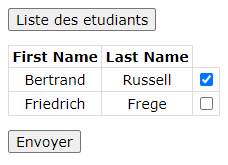
\includegraphics[width=5cm]{assets/attendance.PNG}
            \caption{Page HTML généré par \texttt{RecordAttendance}}
            \label{attendance}        
        \end{center}
    \end{minipage}
\end{figure}

\section{JeSuisEnCours}

Après quelques semaines, nous nous sommes rendus compte que la direction du projet était incompatible avec les exigences administratives. En effet, l'application prévoyait un simple appel du professeur, or l'étudiant doit personnellement attester de sa présence en émargeant un document. Il donc été décidé d'abandonner le projet intiale Attendance pour se tourner vers une application JeSuisEnCours, spécialisée dans la digitalisation les feuilles de présences. 

Le but principal du projet est donc devenu la connexion de l'application JeSuisEnCours aux données de l'université, d'une part, pour accéder aux données (annuaires, emploies du temps,...), d'autre part pour gérer les éléments renvoyés par l'application (absence, justificatif,...).

Malheureursement, la crise sanitaire a fortement ralentit les contacts avec l'équipe de JeSuisEnCours et le projet a finalement été abandonné.